\chapter{Integration Notes}

\section{Integration into a Project}
\ifnum \DocumentGroup=1
{There is no need for standard installation procedure for RTA-SUM SUSD. Once RTA-SUM plugin is installed,
RTA-SUM SUSD gets available for being integrated into a project. Create a new RTA-CAR project
in ISOLAR-A/B and select the Model Year (MY) version. Open the RTA Code Generator dialog and enable
RTA-SUM SUSD by choosing the MY selected during the project creation. If the option \textit{Not Configured}
is chosen instead, the module will not be integrated.\newline
Please refer to RTA-SUM plugin Getting Started Guide for more details about how to integrate this
module into a project.}
\else
{
There is no need for standard installation procedure for SUSD. The folder itself contains all the necessary
artifacts to integrate into a project. Dropping the complete folder structure into a BSW configuration
project will enable the user to configure SUSD and generate all the necessary artifacts.
}
\fi

Refer to \href {https://rtahotline.etas.com/confluence/display/RH/RTA-SUM} {RTA-SUM Knowledge Base} for more details about how to integrate this module into a project. 

\section{Prerequisites}
\label{sec:prerequisites}
You shall have the RTA-CAR toolchain installed as the following list and you must be familiar with the AUTOSAR specifications, terminology and methodology,
\input{generated/tables/tools.tex}

\section{Module Dependencies}
\begin{enumerate}
\item \code{RE\_SUSD\_RunCrankManagement} shall be executed before \code{RE\_SUSD\_VehiclePowerMode}.
\item On wakeup, all SWCs shall be indicated through Permit Execution interface, mapping of SWCs to wakeup is not considered.
\item \code{NvM_WriteAll()} will be done for \code{SUSD_WakeUpSrcTimeInfo} by NvM module.
\end{enumerate}


\section{Configuring RTA-SUM SUSD}
Once the complete package has been added to a BSW project, an additional module SUSD should
appear. From here you can open and begin configuring the module. Specific description of each
configurable parameter is available in the “Description” view of 
\ifnum \DocumentGroup=0
{ISOLAR-AB}
\else
{ISOLAR-A with BCT add-on}
\fi
 when a parameter is selected.
Refer to Section \ref{chap:conf} for more details about RTA-SUM SUSD configuration.

\subsection{Port Connections and timer configuration}
Ensure that the DRE runnables and related ports are connected and well configured so that the refreshes timers will be restored for the \emph{ShutdownPermission}.
The main timing parameters to configure for the behaviour described in the Design Document are:
\begin{itemize}
\item \textbf{SUSD\_t\_Shoutdown\_Refresh}: interval (in seconds) within which each SW-C must send the refresh on its ShutdownPermission interface.
\item \textbf{SUSD\_t\_Force\_shutdown\_Wait}: interval (in seconds) that SUSD waits, starting from the absence of any \emph{PermitExecution}, before requesting Shutdown from BswM.
\end{itemize}
These parameters must be set in the SUSD configuration panel (see Chapter \ref{chap:conf}) to ensure temporal consistency between DRE runnables and SUSD internal timers.

\section{Generating Artifacts}
\label{sec:Artifacts}
Generating the C/H/SWCD files from your configuration is similar to other BSW modules delivered
from ETAS. The Code Generation perspective of the 
\ifnum \DocumentGroup=0
{ISOLAR-AB}
\else
{ISOLAR-A with BCT add-on}
\fi
should present the user with a dialog
to select specific module within the project to generate.
\ifnum \DocumentGroup=1{
%Nothing}
\else{
Either a Partial Build or Full Build can be used, depending on the needs of the user.}
\fi
In case of any configuration errors present in SUSD, the
console window will output a description of any errors found during generation. Further, when the
user is configuring the module, the Problems Log will show any active errors in the configuration of
SUSD. A third visual aid is the appearance of red X’s in the configuration view over items which are
invalid. Simply hovering over these X’s will provide the user a description of the problem. These are
static validations. \\

After generating the SUM files, execute the MemMap tool to generate memory mapping file of the module (\file{SUM\_SUSD\_MemMap.h}).

\section{Configuring the RTE}

After the user has configured and generated the artifacts for SUSD, the output SWCD file \linebreak(\file{SUM\_SUSD\_SWCD.arxml}) can be used for the RTE configuration.
This is a complete SWC description per the AUTOSAR standard of all the users configured ports and interfaces required for the project specific configuration.
This SWCD is a standard ASW component and not a module description.
Therefore, there are no special considerations to be taken into account when configuring the RTE.
It is recommended that if specific changes are required to the SWCD, the user does not manually edit this file, rather update and regenerate the configuration with the required changes.

Note: RTE command used for RTE generation

\begin{rtecommandline}
-nts --samples=memmap --os-define-osenv=RTAOS40 --exclusive-area-optimization=enable --os-output-param=all --have-64bit-int-types=1 --strict-unconnected-rport-check=off -tsl=256
\end{rtecommandline}

% In order to fulfill the requirement to store the SumSUSDInitValue in memory, AUTOSAR typed Per Instance Memory is used for storing this data in non-volatile memory.
% Therefore, it is assumed the user will configure the NVM stack to support this required information.
% Further, it is expected that during shutdown, the appropriate BSW services will write that specific NVM block to persistent storage.

\chapter{Module Configuration}\label{chap:conf}
This section is intended to provide guidelines for RTA-SUM SUSD configuration.

\section{Configuration Parameters}
\label{sec:confparams}
RTA-SUM SUSD parameters are divided in four containers: SUSDConfigSet, SUSDGeneral, SUSDWakeUpRelation and SUSDSUMInterfaces. 

% \begin{figure}[htp]
% 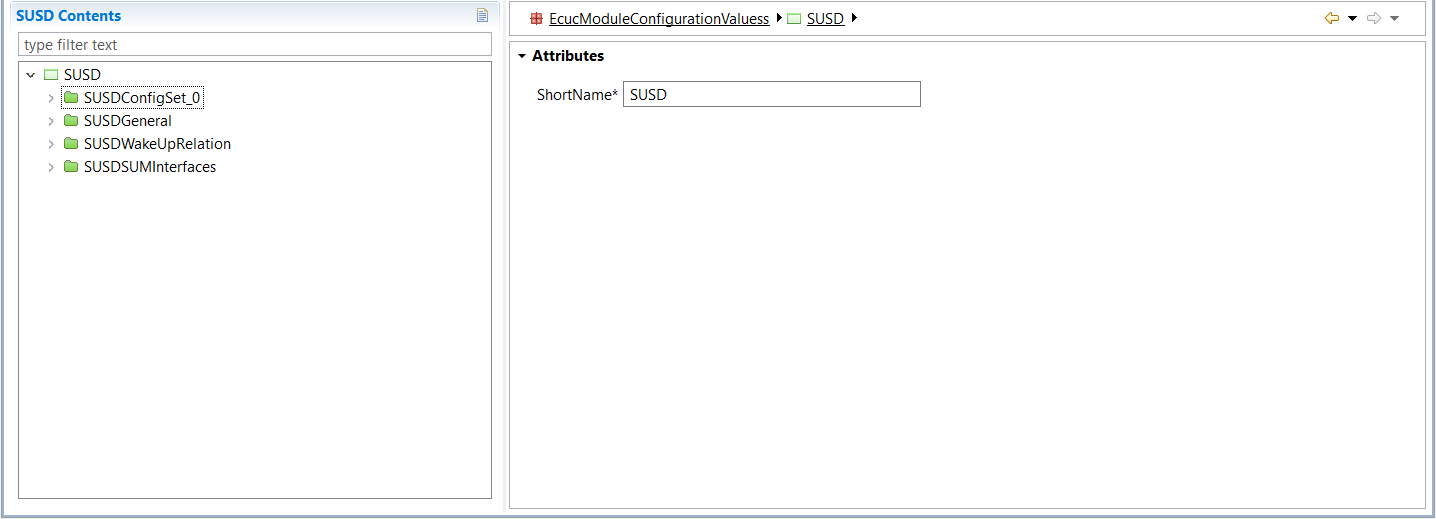
\includegraphics[width=\textwidth]{images/general.png}
% \caption{Containers for RTA-SUM SUSD configuration}\label{fig:containers}
% \end{figure}

\subsection{SUSDConfigSet}
This container (Figure \ref{fig:SUSDConfigSet0}) includes the configuration
parameters and sub containers of the SUSD
module supporting multiple SWC configuration
sets.

\begin{figure}[htp]
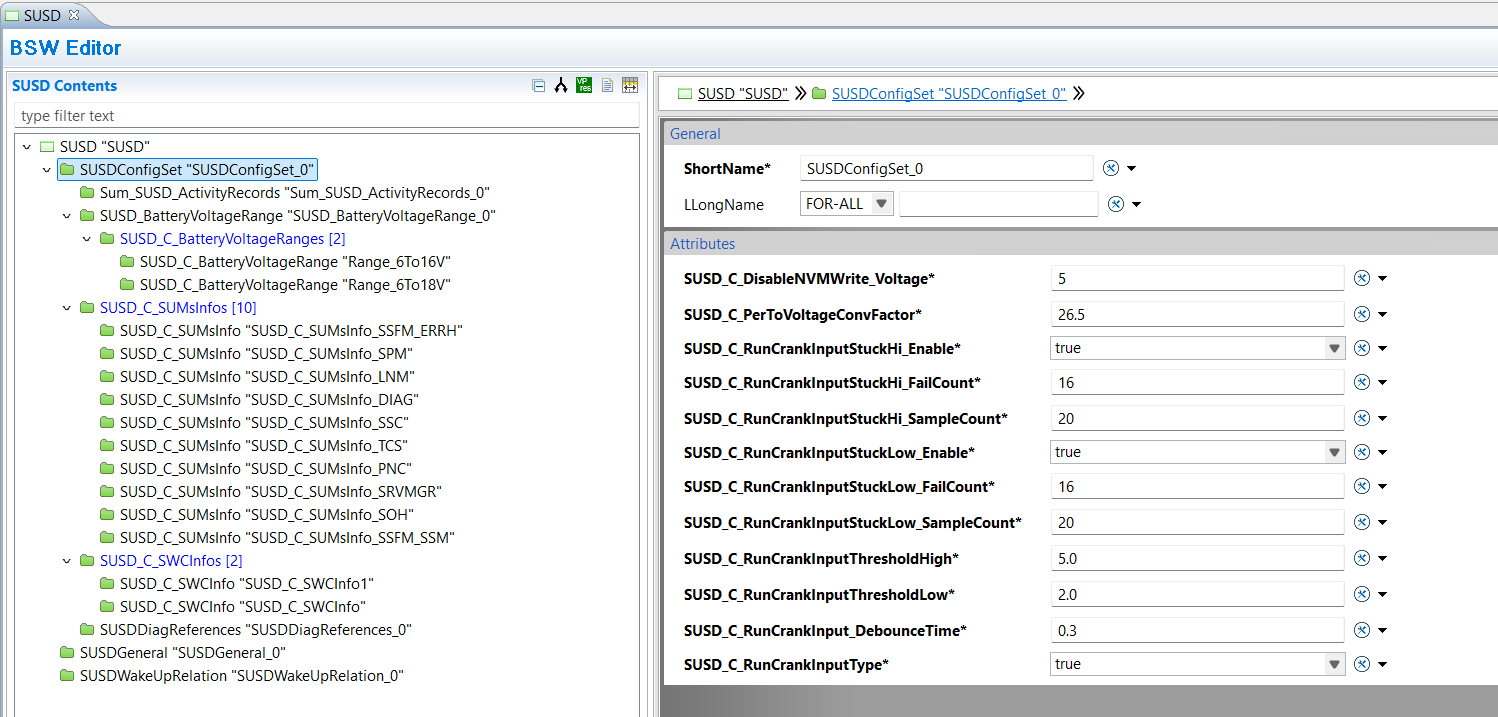
\includegraphics[width=\textwidth]{images/SUSDConfigSet_0.png}
\caption{SUSDConfigSet container}\label{fig:SUSDConfigSet0}
\end{figure}

\textbf{SUSD\_C\_DisableNVMWrite\_Voltage}\newline
A calibration parameter which indicates to SW-Cs to disable any NVM write processes if the battery voltage is below this value. This parameter is used together with the Battery Voltage Sensor Status signal to control the \textit{DisableNvMWrite} signal. Please refer to subsection \ref{subsec:battVltgSnsrStsAvl} for more details.

\textbf{SUSD\_C\_PerToVoltageConvFactor}\newline
A calibration parameter, which represents the Percentage to Voltage Conversion Factor. 

\textbf{SUSD\_C\_RunCrankInputStuckHi\_Enable}\newline
When it is set to true, this calibration parameter enables the Run Crank Stuck High Diagnostic. Otherwise, it disables the Run Crank Stuck High Diagnostic.

\textbf{SUSD\_C\_RunCrankInputStuckHi\_FailCount}\newline
This calibration defines the maximum value of the fault maturation's failure counter for Run Crank Input Stuck High.

\textbf{SUSD\_C\_RunCrankInputStuckHi\_SampleCount}\newline
This calibration defines the maximum value of the fault maturation's sample counter for Run Crank Input Stuck High.

\textbf{SUSD\_C\_RunCrankInputStuckLow\_Enable}\newline
When it is set to true, this calibration parameter enables the Run Crank Stuck Low Diagnostic. Otherwise, it disables the Run Crank Stuck Low Diagnostic.

\textbf{SUSD\_C\_RunCrankInputStuckLow\_FailCount }\newline
This calibration defines the maximum value of the fault maturation's failure counter for Run Crank Input Stuck Low.

\textbf{SUSD\_C\_RunCrankInputStuckLow\_SampleCount }\newline
This calibration defines the maximum value of the fault maturation's sample counter for Run Crank Input Stuck Low. 

\textbf{SUSD\_C\_RunCrankInputThresholdHigh }\newline
This calibration parameter defines the threshold voltage for the Run Crank Input High (RunCrank Active High) determination.

\textbf{SUSD\_C\_RunCrankInputThresholdLow  }\newline
This calibration parameter defines the threshold voltage for the Run Crank Input Low (RunCrank Active Low) determination.

\textbf{SUSD\_C\_RunCrankInput\_DebounceTime  }\newline
Time expressed in seconds, which represents the duration related to the Analog or Digital Run Crank Input (Low/High) determination.

\textbf{SUSD\_C\_RunCrankInputType    }\newline
This calibration is used to determine the Run Crank Input Type (DISCRETE/ANALOG). By default, the Run Crank Input Type is DISCRETE.

\subsubsection{SUSDConfigSet/SUSD\_C\_SWCInfo}
\label{subsection:SUSDSWCInfo}
This section refer to the SUSD\_C\_SWCInfo sub-container  of SUSDConfigSet.

\textbf{SUSD\_SWCName}\newline
A string to indicate the SWC name for interface to map the ports in SWC-D.

\textbf{SUSD\_C\_ShutdownPermControl}\newline
A boolean calibration parameter for each shutdown permission interface to control the processing of its permissions.

\textbf{SUSD\_BatteryVoltageRangeRef}\newline
Reference to a battery voltage range in SUSD\_BatteryVoltageRange container.

\textbf{SUSD\_C\_SWCs\_SpecificWkSrcId}\newline
Reference to a wakeup source. This parameter defines the identifier of this wakeup source.

\subsubsection{SUSDConfigSet/SUSD\_C\_SUMsInfo}
\label{subsection:SUSDSUMsInfo}
This section refers to the SUSD\_C\_SUMsInfo sub-container of SUSDConfigSet which contains configuration parameters for SUM (System Unit Manager) components that SUSD interfaces with.

\textbf{SUSD\_SUMsName}\newline
This enumeration parameter defines the type of SUM component that SUSD will interface with. Available options include:
\begin{itemize}
\item SUM\_SPM 
\item SUM\_LNM   
\item SUM\_SSFM-ERRH
\item SUM\_SSFM-SSM
\item SUM\_SSC 
\item SUM\_PNC 
\item SUM\_DIAG
\item SUM\_TCS
\item SUM\_SRVMGR
\item SUM\_SOH
\end{itemize}

\textbf{SUSD\_PermitExecution}\newline
Boolean parameter that enables or disables the Permit Execution Interface to the selected SUM component.

\textbf{SUSD\_ShutdownPermission}\newline
Boolean parameter that enables or disables the Shutdown Permission Interface to the selected SUM component.

\textbf{SUSD\_SUMs\_SpecificWkSrcId}\newline
Reference to a wakeup source. This parameter defines the identifier of the wakeup source associated with the SUM component.

\subsubsection{SUSDConfigSet/SUSDDiagReferences}
\label{sec:DcmRef}
The SUSDDiagReferences sub-container includes the configuration parameters related to diagnostic services provided by RTA-SUM SUSD.

\textbf{SusdEcuWakeupDetectionRecordsDidRef}\newline
Reference to DID 0xF09E "ECU Wakeup Detection Records" configuration in the Dcm module.

\textbf{SusdRid41ARef}\newline
Reference to RID 0x41A "Clear ECU Wakeup Detection Records" configuration in the Dcm module.

\textbf{Did\_E0D7\_Reference}\newline
Reference to DID 0xE0D7 "Wakeup and Off Power Mode Activity Records" configuration in the Dcm module.

\textbf{Did\_F088\_Reference}\newline
Reference to DID 0xF088 "Control Module Input Power" configuration in the Dcm module. This DID always uses asynchronous interface with DCM.

\textbf{Did\_F089\_Reference}\newline 
Reference to DID 0xF089 Application Shutdown Prohibit, that contains the current internal value of the permission for the ECU to shutdown.

\subsubsection{SUSDConfigSet/SUSD\_BatteryVoltageRange}
\label{subsection:BatteryVoltageRange}
SUSD implements the P-Port PP\_SUSD\_DefaultBatteryVoltage\_MintoMax\_9Vto16V which is associated to the defaul battery voltage range 9V-16V. The hysteresis of this voltage range can be configured through the configuration parameters SUSD\_C\_DefaultUnderVoltage\_hysteresis and \\ SUSD\_C\_DefaultOverVoltage\_hysteresis described below. \newline

\textbf{SUSD\_C\_DefaultUnderVoltage\_hysteresis}\newline
This parameter represents the hysteresis (in volts) for the under voltage range and only used with 9V-16V.

\textbf{SUSD\_C\_DefaultOverVoltage\_hysteresis}\newline
This parameter represents the hysteresis (in volts) for the over voltage range and only used with 9V-16V.

If different battery voltage ranges are needed, one or more SUSD\_C\_BatteryVoltageRange \\ sub-containers could be added, one per each Battery Voltage Range required. A P-port will be generated per each Battery Voltage Range configured. \\ 
Each sub-container will include the parameters related to the specific Battery Voltage Range: 

\textbf{SUSD\_BatteryVoltageRange\_Max}\newline
The maximum voltage in range.

\textbf{SUSD\_BatteryVoltageRange\_Min}\newline
The minimum voltage in range.

\textbf{SUSD\_C\_UnderVoltage\_hysteresis}\newline
This parameter represents the hysteresis (in volts) for the under voltage range.

\textbf{SUSD\_C\_OverVoltage\_hysteresis}\newline
This parameter represents the hysteresis (in volts) for the over voltage range.

As mentioned in subsection \ref{subsection:SUSDSWCInfo} SUSDConfigSet/SUSD\_C\_SWCInfo, the SW-C shall be linked to the Battery Voltage Range by adding the corresponding Battery Voltage Range reference in the \\ SUSD\_C\_SWCInfo sub-container. If not reference is configured, the default Battery Voltage Range will be used.

\subsection{SUSDGeneral}
\label{subsection:SUSDGeneral}
This container (Figures \ref{fig:SUSDGeneral} and \ref{fig:SUSDGeneral_Refs}) includes the general configuration parameters of RTA-SUM SUSD.

\begin{figure}[H]
\centering
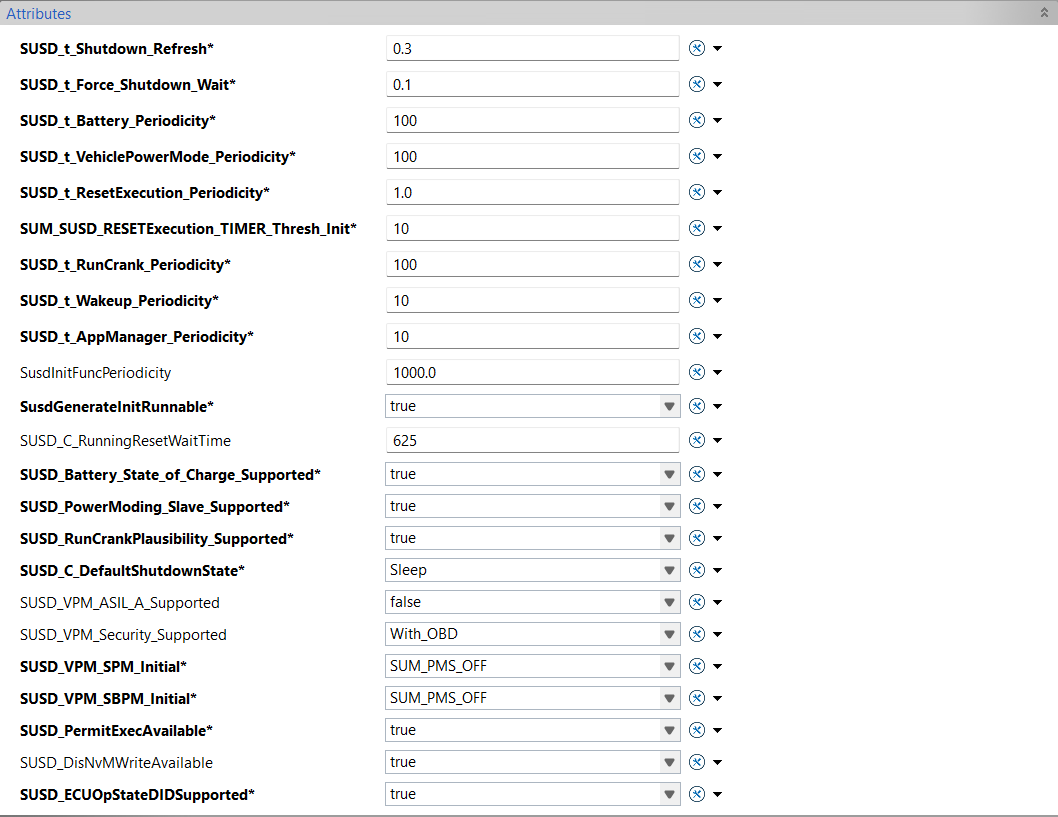
\includegraphics[width=0.9\textwidth]{images/SUSDGeneral.png}
\caption{SUSDGeneral container}\label{fig:SUSDGeneral}
\end{figure}

\begin{figure}[H] 
\centering
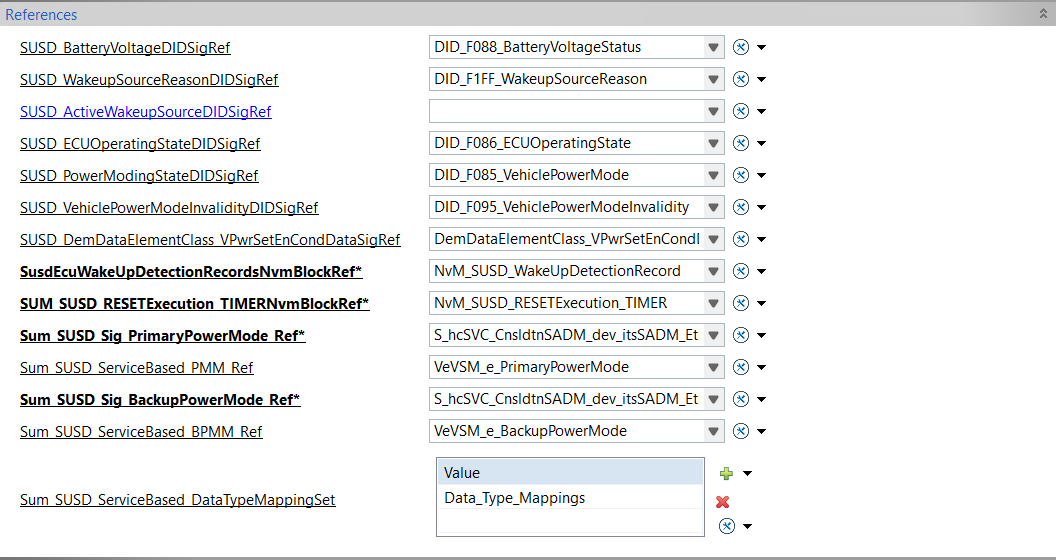
\includegraphics[width=0.9\textwidth]{images/SUSDGeneral_Refs.png}
\caption{SUSDGeneral container - References}\label{fig:SUSDGeneral_Refs}
\end{figure}

\textbf{SUSD\_t\_Shutdown\_Refresh}\newline
Time (in seconds), for which a SW-C with a ShutdownPermission interface, shall refresh its signal for that interface. 

\textbf{SUSD\_t\_Force\_Shutdown\_Wait}\newline
Time in seconds (greater than zero), which SUSD shall wait before requesting Shutdown from BswM, after indicating to all SW-Cs with PermitExecution interface to Shutdown. 

\textbf{SUSD\_t\_Battery\_Periodicity }\newline
Time (in milliseconds), for the periodicity of notifying SW-C of changes to the Battery Monitors.

\textbf{SUSD\_t\_VehiclePowerMode\_Periodicity }\newline
Time (expressed in milliseconds), for the periodicity of notifying SW-C of changes to the Vehicle Power Mode.

\textbf{SUSD\_t\_RunCrank\_Periodicity}\newline
Time (expressed in milliseconds), for the periodicity of notifying SW-C of changes to the Run Crank.

\textbf{SUSD\_t\_Wakeup\_Periodicity}\newline
Time in milliseconds, for the periodicity of Wake up polling.

\textbf{SUSD\_PowerModing\_Slave\_Supported}\newline
This parameter shall be true if the ECU is not the Power Mode Master, false if the ECU is the Power Mode Master.

\textbf{SUSD\_RunCrankPlausibility\_Supported}\newline
This parameter shall be true if the Run Crank Input is available from one of the software component, false if the RunCrank Input is not available from any of the software component.

\textbf{SUSD\_C\_DefaultShutdownState}\newline
This parameter represents the default ECU operation state when shutting down: Off or Sleep.

\textbf{SUSD\_VPM\_ASIL\_A\_Supported }\newline
This parameter shall control the determination of Vehicle Power Mode at ASIL A or QM level. If set to False, then VPM shall be calculated without Failed Safety signals.

\textbf{SUSD\_VPM\_Security\_Supported }\newline
This parameter shall control the determination of Vehicle Power Mode either NoT\_Applicable or with OBD or with Cybersecurity or without Cybersecurity.Then VPM shall be calculated with or without Failed Security signals.

\textbf{SUSD\_VPM\_SPM\_Initial}\newline
This parameter represents the initial value for System Power Mode used for Vehicle Power Mode determination when a valid System Power Mode has not been received yet.

\textbf{SUSD\_VPM\_SBPM\_Initial }\newline
This parameter represents the initial value for System Backup Power Mode used for Vehicle Power Mode determination when a valid System Backup Power Mode has not been received yet.

\textbf{SUSD\_PermitExecAvailable }\newline
A parameter for Permit Execution Interface for this SWC. 

\textbf{SUSD\_ECUOpStateDIDSupported}\newline
This parameter was created to provide the option to choose the ECU Operating State DID as optionals.

\textbf{SUSD\_Battery\_State\_of\_Charge\_Supported}\newline
This parameter must be set equal to true if the ECU has an input which monitors the vehicle battery state of charge.

\textbf{SUM\_SUSD\_RESETExecution\_TIMER\_Thresh\_Init}\newline
This parameter represents the initial value of the Calibration parameter SUM\_SUSD\_RESETExecution\_ TIMER\_Thresh.

\textbf{SUSD\_t\_ResetExecution\_Periodicity}\newline
Time (expressed in milliseconds), for the periodicity of Reset Execution and Running Reset handling. 
Please note that, in order to have an exact timing without any drift or missing detection, the \code{SUSD\_C\_RunningResetWaitTime} and \code{SUM\_SUSD\_RESETExecution\_TIMER\_Thresh\_Init} parameters
and their corresponding calibration values should be divisible by the periodicity. 
The SUM generator will check this condition during the generation with the default values set for the calibration parameters. However, it is the user's responsibility to keep this condition valid during the runtime 
by using compatible calibration parameter values. Otherwise, the timely handling of the related events is not guaranteed.

\textbf{SUSD\_BatteryVoltageDIDSigRef }\newline
Reference to DID for Battery Voltage Signal.

\textbf{SUSD\_WakeupSourceReasonDIDSigRef}\newline
Reference to DID for Wakeup Source Reason Signal.

\textbf{SUSD\_ActiveWakeupSourceDIDSigRef}\newline
Reference to DID for Active Wakeup Source(s) Signal.

\textbf{SUSD\_ECUOperatingStateDIDSigRef}\newline
Reference to DID for ECU Operating State Signal.

\textbf{SUSD\_PowerModingStateDIDSigRef}\newline
Reference to DID for Power Moding State Signal.

\textbf{SUSD\_VehiclePowerModeInvalidityDIDSigRef}\newline
Reference to DID for Vehicle Power Mode Invalidity Signal.

\textbf{SUSD\_DemDataElementClass\_VPwrSetEnCondDataSigRef}\newline
Reference to Dem Data Element Class for Vehicle Power Set Enable Condition Data Signal.

\textbf{SusdEcuWakeUpDetectionRecordsNvmBlockRef}\newline
Reference to NVM Block Descriptor configuration for storing ECU Wakeup Detection Records.

\textbf{SUSD\_RESETExecution\_TIMERNvmBlockRef}\newline
This parameter represents the reference to the NVM Block Descriptor configuration used for storing SUM\_SUSD\_RESETExecution\_TIMER.

\textbf{SUSD\_C\_RunningResetWaitTime}\newline
This parameter represents the wait time after running reset occurs before going to fail soft action.

\textbf{SusdGenerateInitRunnable}\newline
The parameter shall generate SUSD init runnable if it is configured as TRUE. Otherwise the SUSD\_Init() function shall be called by a BswM action list during startup.

\textbf{SusdInitFuncPeriodicity}\newline
The parameter shall define the period in milliseconds that configures the runnable init function periodicity. This parameter is required when SusdGenerateInitRunnable is set to TRUE.

\textbf{Sum\_SUSD\_Sig\_PrimaryPowerMode\_Ref}\newline
The parameter represents the reference to the primary power mode signal or group signal used for Vehicle Power Mode determination.

\textbf{Sum\_SUSD\_Sig\_BackupPowerMode\_Ref}\newline
The parameter represents the reference to the backup power mode signal or group signal used for Vehicle Power Mode determination.

\textbf{Sum\_SUSD\_ServiceBased\_PMM\_Ref}\newline
The parameter represents a reference to the service-based PMM interface used for Vehicle Power Mode determination.

\textbf{Sum\_SUSD\_ServiceBased\_BPMM\_Ref}\newline
The parameter represents a reference to the service-based BPMM interface used for Vehicle Power Mode determination.

\textbf{Sum\_SUSD\_ServiceBased\_DatatypeMappingSet}\newline
The parameter represents the reference to the data type mapping set used for service-based PMM and BPMM interfaces.

\subsection{SUSDWakeUpRelation/SUSD\_WakeUpSourceIds}
This container (Figure \ref{fig:SUSDWakeUpRelation}) includes a list of Wakeup Source
identifiers that are needed to refer to indicate the
Permit Execution to SUMs.

\begin{figure}[htp]
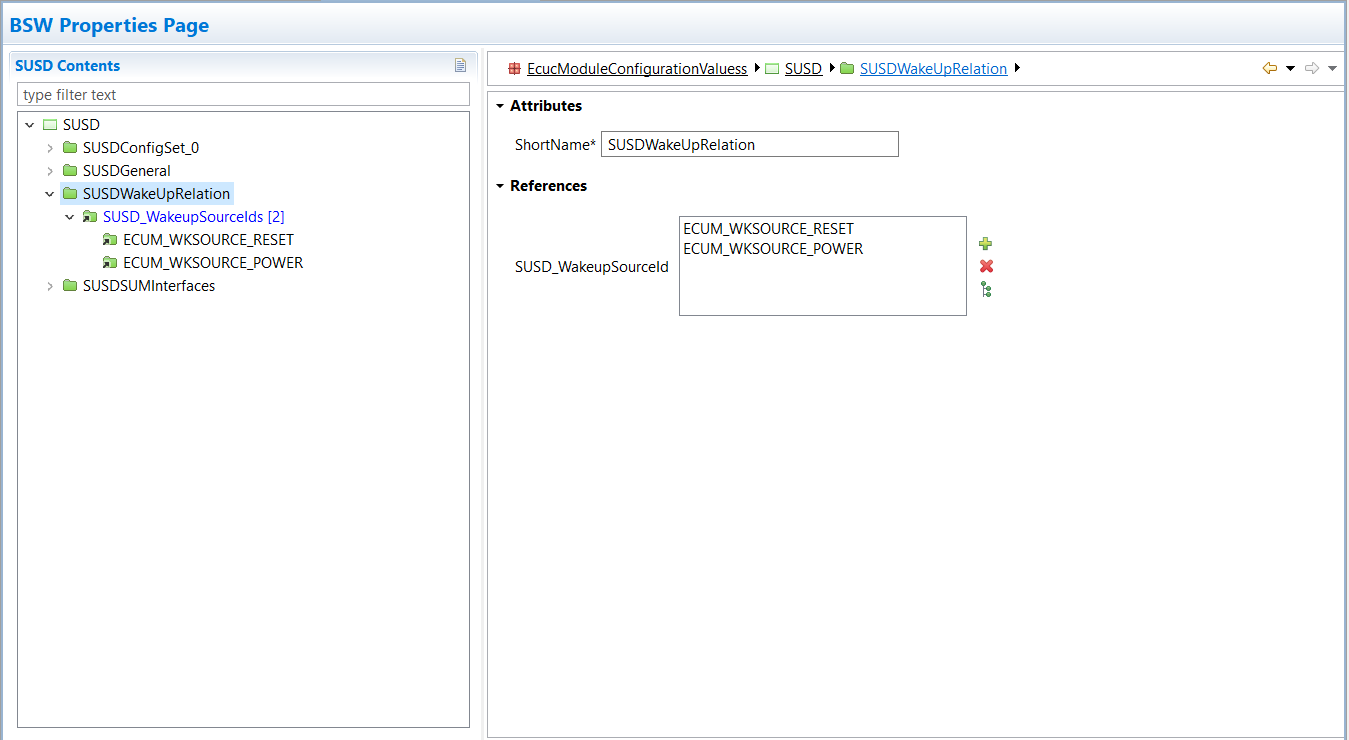
\includegraphics[width=\textwidth]{images/SUSDWakeUpRelation.png}
\caption{SUSDWakeUpRelation container}\label{fig:SUSDWakeUpRelation}
\end{figure}

\textbf{SUSD\_WakeupSourceId}\newline
This parameter defines the identifier of this wakeup source.

\section{Configuration Hints}

\subsection{VehicleBatteryVoltage}
\label{subsec:vehBatVolt}
VehicleBatteryVoltage is an \textit{ApplicationDatatype} mapped to an \textit{ImplementationDatatype} and 'uint16' basetype. So every instance where VehicleBatteryVoltage is used, shall require \underline{DatatypeMappingSet} - \code{DTMS_SUSD_VehcleBatryVlg} added to DatatypeMappings of the \underline{using} SWC.

SUSD reads Battery Voltage value from SW-C through a rport \textbf{\textit{RP\_SUSD\_VehicleBatteryVoltage}}. The \textbf{decivolt input} as integer unsigned (uint16) is required so
the integrator is highly recommended to change the input port prototype. Define CompuMethods if they are needed.

\subsection{BattVltgSnsrStsAvl}
\label{subsec:battVltgSnsrStsAvl}
SUSD provides the required port \textbf{\textit{RP\_SUSD\_BattVltgSnsrStsAvl}} \\(interface \code{SUSD\_BattVltgSnsrStsAvl}, data element \code{BattVltgSnsrStsEnum}) to read the Battery Voltage Sensor Status from the Tier1 SW-C. The Tier1 shall implement the corresponding provided port (PP). This port is mandatory and is used together with \textit{RP\_SUSD\_VehicleBatteryVoltage} to control the \textbf{DisableNvMWrite} signal:
\begin{itemize}
\item SUSD sets \textit{DisableNvMWrite} = \textit{FALSE} (write allowed) only if: \\voltage $\geq$ \code{SUSD\_C\_DisableNVMWrite\_Voltage} \\ \textbf{AND} \code{BattVltgSnsrStsEnum} == 2 (\textit{Battery\_Voltage\_Available}).
\item If either condition is not met, \textit{DisableNvMWrite} = \textit{TRUE} and all SUM SW-Cs shall inhibit direct NvM write calls.
\end{itemize}

\textbf{Note on WriteAll at shutdown:} When \textit{DisableNvMWrite} is \textit{TRUE}, SUM SW-Cs update the NvM RAM mirror and call \code{NvM\_SetRamBlockStatus()} to flag the block as modified. The NvM blocks shall be configured with \textit{WriteAll} support so that at ECU shutdown the BswM invokes \code{NvM\_WriteAll()} and the modified blocks are persisted. SUSD cannot control this WriteAll trigger; it is the Tier1 responsibility to configure the BswM conditions, actions, and rules to prevent the write when battery voltage is insufficient at shutdown.

\subsection{BatteryVoltage\_Actual}
BatteryVoltage\_Actual is an \textit{ApplicationDatatype} mapped to an \textit{ImplementationDatatype} and 'uint16' basetype. So every instance where BatteryVoltage\_Actual is used, shall require \underline{DatatypeMappingSet} - \code{DTMS_SUSD_VehcleBatryVlg} added to DatatypeMappings of the \underline{using} SWC.


BatteryVoltage DID configuration is \textit{\textbf{OPTIONAL}}.

\subsection{System Power Mode}
\label{sec:pmm}
SUM\_SUSD supports both signal-based and service-based configurations for System power mode signal.

SUM\_SUSD needs to read and evaluate the System Power Mode signal.
To do that, it reads the value of \textit{SystemPowerMode} signal via the RTE port interface RP\_Com\_SUSD\_VeVSM\_e\_PrimaryPowerMode.

For this purpose, the signal must be referenced in the Sum\_SUSD\_Sig\_PrimaryPowerMode\_Ref parameter.

\subsubsection{Service-Based SystemPowerMode Configuration}
\label{sec:servicebasedpmm}
For service-based SystemPowerMode, SUM\_SUSD requires additional configuration to  properly reference the system data type mappings and implementation data type elements. The following parameters enable this functionality:

\textbf{SUM\_SUSD\_Sig\_SystemPowerMode\_Ref Configuration:}

This choice reference parameter configures the reference to the Com Signal for System Power Mode. The signal can be configured as either:
\begin{itemize}
  \item Service Based (ComSignal)
	\item Signal Based (ComSignal)
	\item Signal Based (ComGroupSignal)
\end{itemize}

\textbf{SUM\_SUSD\_ServiceBased\_DataTypeMappingSet Configuration:}

This foreign choice reference parameter configures the reference to the DATA-TYPE-MAPPING-SET in the system extract. The parameter must be configured to point to the correct data type mapping set used for service-based operations including PMM and BPMM. This parameter supports multiple references (UPPER-MULTIPLICITY-INFINITE) to accommodate different data type mapping sets for various service-based functionalities.

\textbf{SUM\_SUSD\_ServiceBased\_PMM\_Ref Configuration:}

This foreign reference must be configured to the specific IMPLEMENTATION-DATA-TYPE-ELEMENT that contains the service-based PMM functionality within the software architecture packages. This reference establishes the connection between the SUSD module and the system's PMM implementation data types.

\begin{figure}[]
	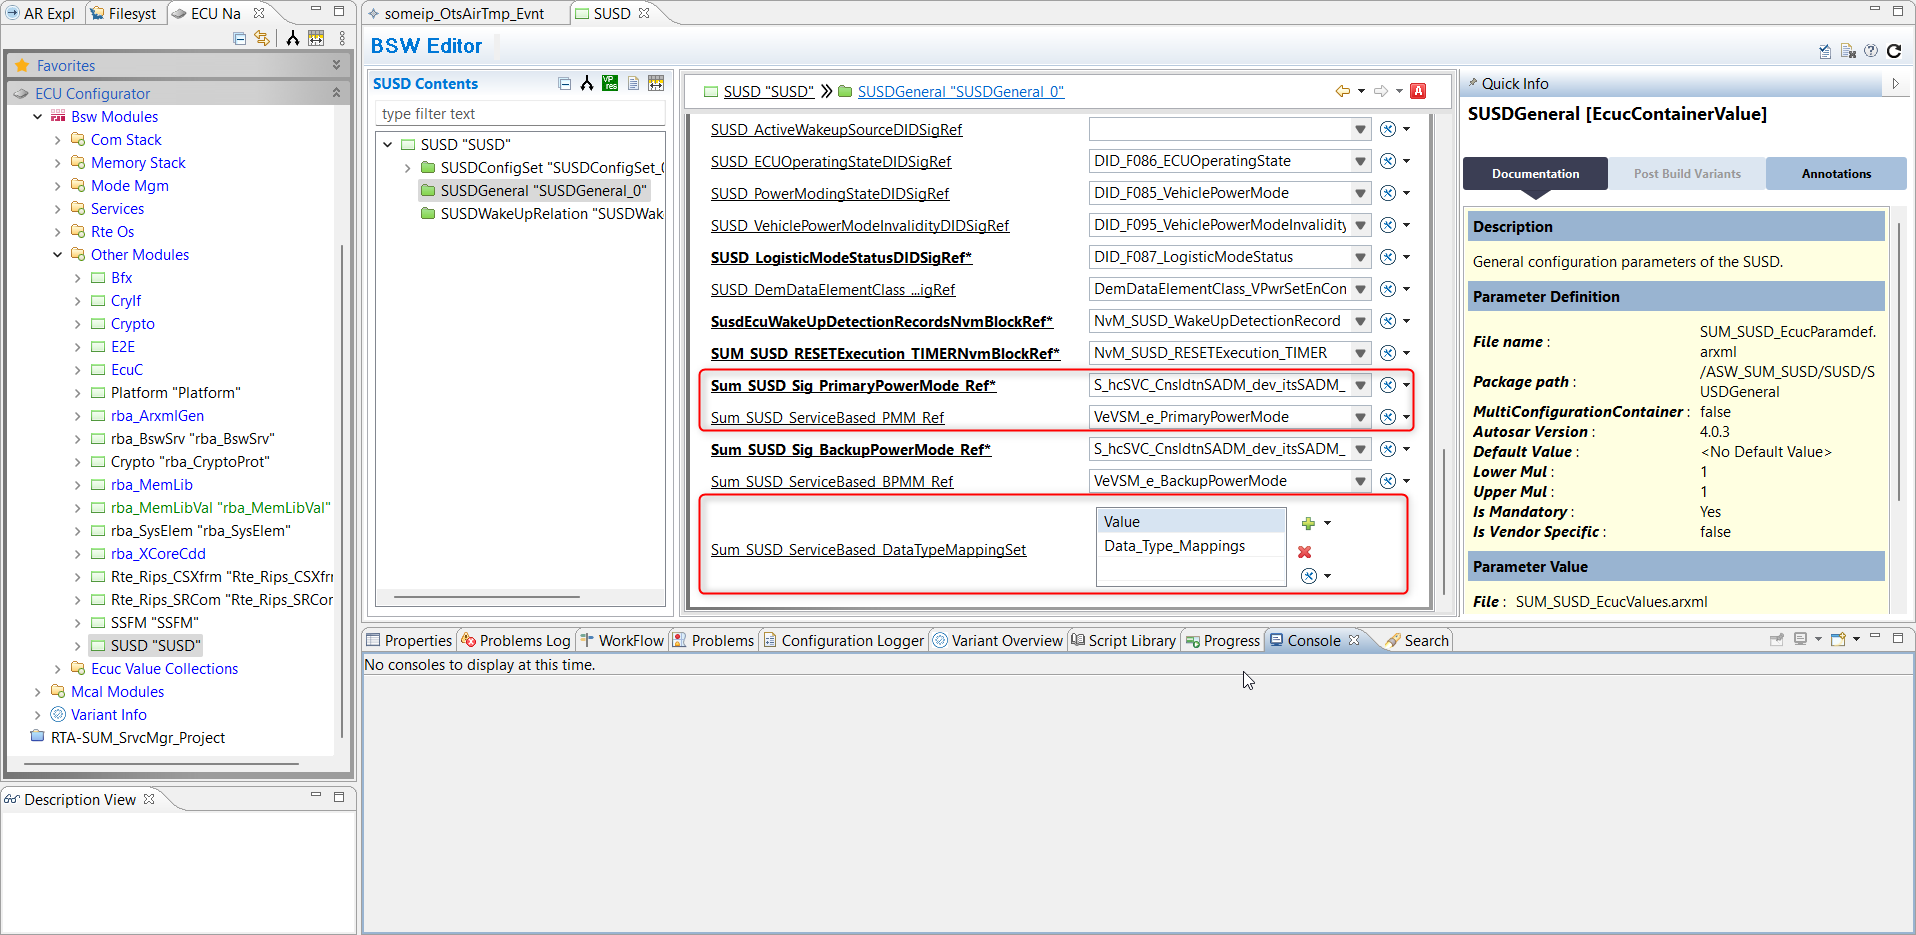
\includegraphics[width=1\textwidth]{images/PMM_ServiceBasedConfigurations.png}
	\caption{ RTA-SUM SUSD Service-Based PMM}
\end{figure}

\textbf{Configuration Dependencies:}
When configuring service-based PMM operations, ensure that:
\begin{itemize}
	\item The \texttt{SUM\_SUSD\_ServiceBased\_DataTypeMappingSet} references a valid DATA-TYPE-MAPPING-SET in the system extract
	\item The \texttt{SUM\_SUSD\_ServiceBased\_PMM\_Ref} references an existing IDTE (IMPLEMENTATION-DATA-TYPE-ELEMENT) (when using service-based communication)
	\item The referenced implementation data type element is properly defined in the system architecture
	\item The data type mappings are consistent with the system's service-based PMM implementation
	\item The port RP\_Com\_SUSD\_VeVSM\_e\_PrimaryPowerMode is properly connected to the Com module for receiving the PMM signal by mapping 
\end{itemize}

\subsection{Backup Power Mode}
\label{sec:bpmm}
SUM\_SUSD supports both signal-based and service-based configurations for Backup Power Mode signal.

SUM\_SUSD needs to read and evaluate the Backup Power Mode signal for Vehicle Power Mode update.
It reads the value of \textit{BPMM} via the port interface RP\_Com\_SUSD\_VeVSM\_e\_BackupPowerMode.

For this purpose, the signal must be referenced in the SUM\_SUSD\_Sig\_BackupPowerMode\_Ref parameter.

\textbf{SUM\_SUSD\_Sig\_BackupPowerMode\_Ref Configuration:}

This choice reference parameter configures the reference to the Com Signal for Backup Power Mode. The signal can be configured as either:
\begin{itemize}
  \item Service Based (ComSignal)
	\item Signal Based (ComSignal)
	\item Signal Based (ComGroupSignal)
\end{itemize}

The SUM\_SUSD module reads this signal via the RTE port interface to obtain BPMM information for various operations.

\textbf{SUM\_SUSD\_ServiceBased\_BPMM\_Ref Configuration:}

This foreign reference must be configured to the specific IMPLEMENTATION-DATA-TYPE-ELEMENT that contains the service-based Backup Power Mode functionality within the software architecture packages from the System Extract. This reference enables service-oriented communication for BPMM.

\begin{figure}[]
	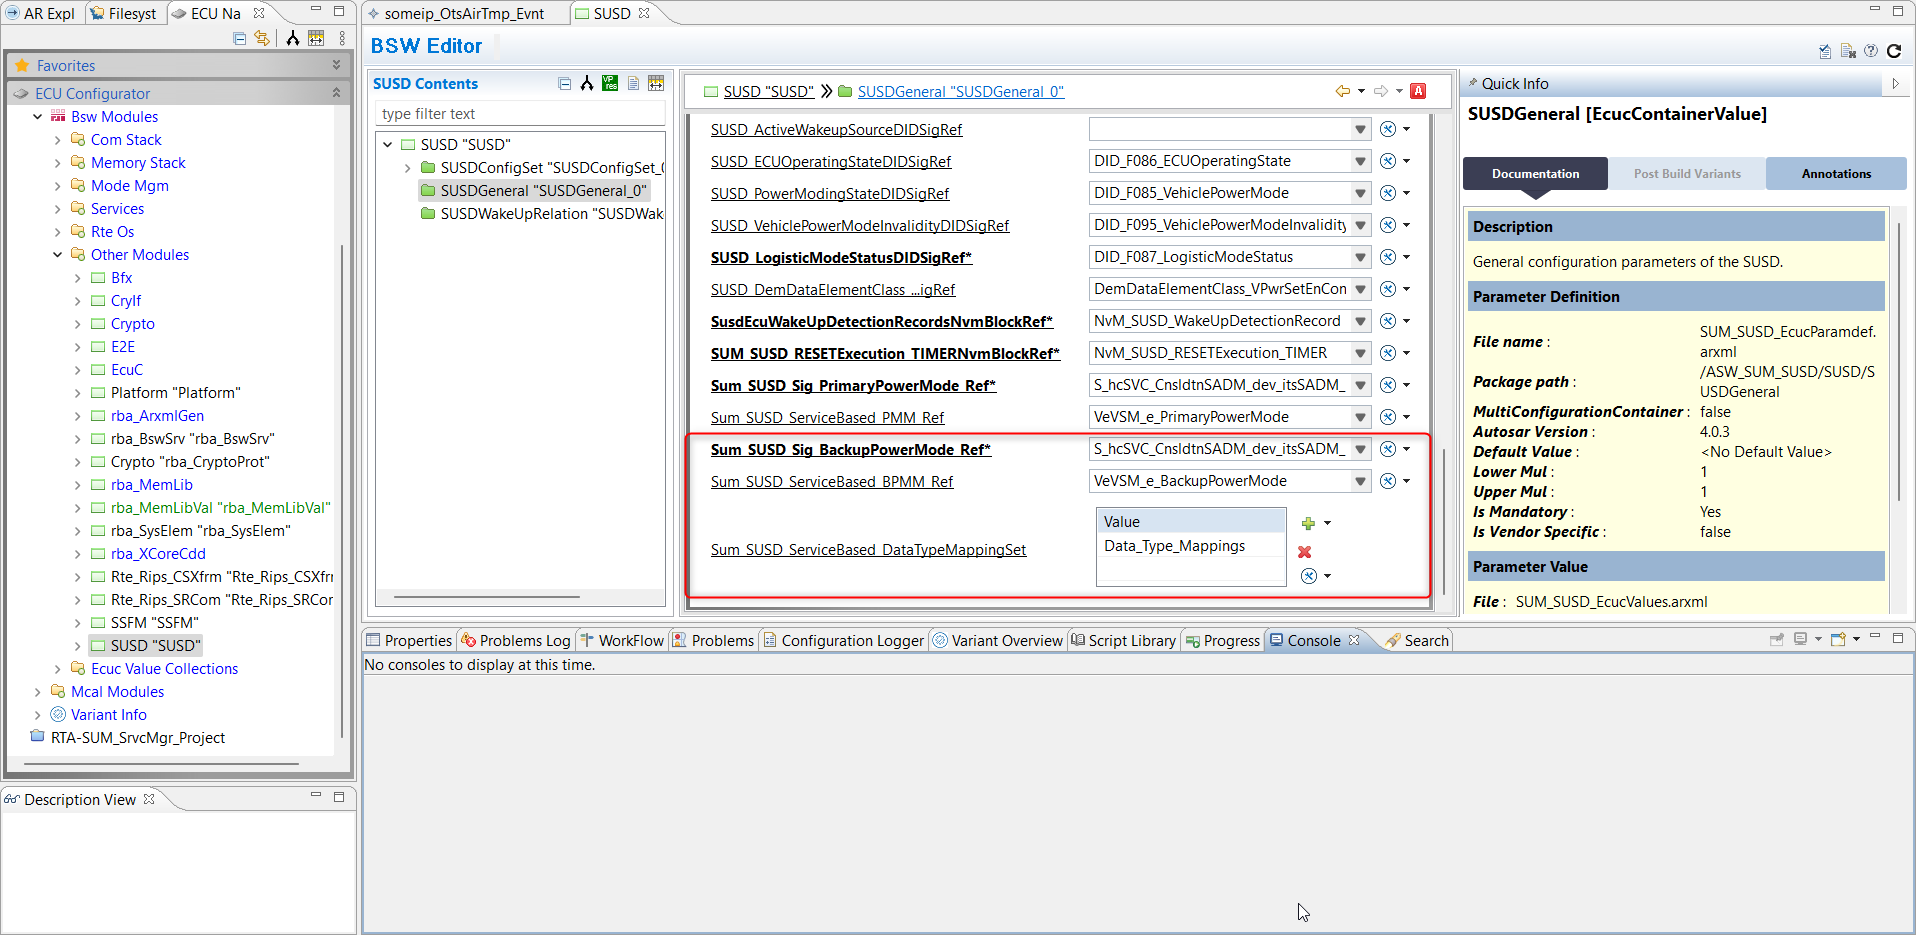
\includegraphics[width=1\textwidth]{images/BPMM_ServiceBasedConfigurations.png}
	\caption{ RTA-SUM SUSD Service-Based BPMM}
\end{figure}

\textbf{Configuration Dependencies:}
When configuring Backup Power Mode operations, ensure that:
\begin{itemize}
	\item The \texttt{SUM\_SUSD\_Sig\_BPMM\_Ref} references a valid ComSignal or ComGroupSignal
	\item The \texttt{SUM\_SUSD\_ServiceBased\_BPMM\_Ref} references an existing IDTE (IMPLEMENTATION-DATA-TYPE-ELEMENT) (when using service-based communication)
	\item The \texttt{SUM\_SUSD\_ServiceBased\_DataTypeMappingSet} includes appropriate data type mapping sets for backup power mode operations
	\item The referenced implementation data type element is properly defined in the system architecture
	\item The Com signal is properly connected to the SUSD required port interface before RTE code generation
\end{itemize}

\textbf{Note - Unified Configuration for Service-Based PMM and BPMM:} 

The \texttt{SUM\_SUSD\_ServiceBased\_DataTypeMappingSet} parameter is used for both Primary Power Mode (PMM) and Backup Power Mode (BPMM) service-based configurations. This unified data type mapping set enables consistent service-based communication for both signal types across the module. 

Additionally, when both PMM and BPMM are provided as service-based signals, the SUSD module can utilize the unified port interface \textit{RP\_Com\_SUSD\_PrimaryPowerMode\_BackupPowerMode} to access both signals through a single interface, providing simplified configuration and unified access.

\textbf{Signal Configuration Summary} 

\begin{table}[]
\centering
\begin{tabular}{|l|l|l|l|}
\hline
\textbf{Signal} & \textbf{Mode} & \textbf{Category} & \textbf{Type} \\ \hline
\multirow{3}{*}{PMM} & Service-Based & ComSignal & UINT8\_N \\ \cline{2-4} 
 & Signal-Based & ComSignal/ComGroupSignal & UINT8 \\ \hline
\multirow{3}{*}{BPMM} & Service-Based & ComSignal & UINT8\_N \\ \cline{2-4} 
 & Signal-Based & ComSignal/ComGroupSignal & UINT8 \\ \hline
\end{tabular}
\caption{Valid Signal Configurations}
\label{tab:signalconfigs}
\end{table}

\textbf{Key Rules:}
\begin{itemize}
	\item Service-based \textbf{requires} ComSignal with UINT8\_N (ComGroupSignal not allowed)
	\item Signal-based allows ComSignal or ComGroupSignal with fixed-size types
\end{itemize}

\subsection{SUSD Diagnostic Services}
\label{subsection:SUSDDiagnosticServices}
\textbf{ DID 0xF09E}

For the support of DID 0xF09E "ECU Wakeup Detection Records" the user shall provide the reference to:
\begin{itemize}
\item The DID configuration in the Dcm module with the parameter \textit{SUSDConfigSet/SUSDDiagReferences/SusdEcuWakeupDetectionRecordsDidRef};
\item The NVM Block Descriptor configuration in the NvM module with the parameter \textit{SUSDGeneral/SusdEcuWakeUpDetectionRecordsNvmBlockRef} for storing the 10 most recent Wakeup Records. The NVM block length shall be configured to \textbf{90 Bytes} because for each Wakeup Record SUSD stores 4 Bytes for "ECUWakeupDetectionRecord" field and 5 Bytes for "Time Stamp" field (taken from TCS\_SWC\_Clock interface following big endian). The \textbf{NvMRamBlockDataAddress} parameter shall be set to "\textbf{SUSD\_ECUWakeupDetectionRecordsArray}" because SUSD will access the RAM block through a PIM with such name.
\item Make sure that CPU\_BYTE\_ORDER (Platform configuration parameter : PlatformRbCpuByteOrder ) is aligned with the endianness of your CPU
\end{itemize}
After Dcm, NvM, and SUSD generation, the Pports \texttt{PP\_SUSD\_ECUWakeupDetRec\_<DidSignalName>} shall be connected to the appropriate Dcm Rports related to DID 0xF09E. Moreover, the Rport\\ \texttt{RP\_NVM\_SUSD\_NvMServiceECUWakeUpDetectionRecordsBlock} shall be connected to the appropriate NvM Pport related to the Wakeup Records NVM block.

\textbf{ RID 0x41A and DID 0xE0D7}

For the support of RID 0x41A "Clear ECU Wakeup Detection Records" the user shall provide a reference to the RID configuration in the Dcm module with the parameter \textit{SUSDConfigSet/SUSDDiagReferences/SusdRid41ARef}.
After Dcm and SUSD generation, the Pport \texttt{PP\_SUSD\_RoutineServices\_41A} shall be connected to the appropriate Dcm Rport related to RID 0x41A.

In order to enable support of the optional DIDs "Wakeup Source Reason" and \\"Active Wakeup Source(s)", the user shall configure respectively\\ \textit{SUSDGeneral/SUSD\_WakeupSourceReasonDIDSigRef} and\\ \textit{SUSDGeneral/SUSD\_ActiveWakeupSourceDIDSigRef} as per project specific needs.

On shutdown, all fields required by DID 0xE0D7, including Total Activity Timer, Wakeup Counter, and Activity Records, are stored in NVRAM.

\textbf{ DID 0xF089}

To support the DID 0xF089 "Application Shutdown Prohibit", the user shall provide a DcmDspDid reference in \textit{SUSDConfigSet/SUSDDiagReferences/Did\_F089\_Reference}.
Each bit of this DID represents the Shutdown prohibit status of the SWCs configured in the SUSD. The SWCs include both the Swcs configured in the \textit{SUSDConfigSet/SUSD\_C\_SWCInfo} container and the Sum modules.
In addition, the \textbf{RE\_DID\_F089\_ReadData} runnable, which enables the read operation to populate the DID, will first process the Sum modules and then the Swcs, if configured.

\subsection{Wakeup detection}
To properly detect the activation and deactivation of wakeups, the users should configure the wakeup source, and they should set two rules for each wakeup source. 
In particular, the first rule should invoke the callout function "SUSD\_UpdatedWakeupSource" when the corresponding wakeup channel status is set to two (VALIDATED). 
Similarly, the second rule should invoke the callout function "SUSD\_UpdatedWakeupSource" when the corresponding wakeup channel status is set to zero (NONE). 
Both the callout functions require as input parameter the current status of the wakeups in the ECU. 
The user can retrieve the current wakeups status by using the "EcuM\_GetValidatedWakeupEvents" API. 
To guarantee proper behaviour of SUM\_SUSD, the user should configure the Wakeup Source IDs according to the specifications (SDV-6001).


\subsection{Battery State of Charge Monitoring}
To monitor the battery state of charge, the configuration parameter SUSD\_Battery\_State\_of\_Charge \_Supported must be equal to true.
In fact, the VehicleBatteryStateOfCharge and BatteryCharge\_Disab leWkups interfaces will be generated only when this parameter is set to true.

If this situation represents the users' use case, they should connect the VehicleBatteryStateOfCharge interface to the SWC which is responsible for reading the state of charge (the interface requires a boolean input).
Similarly, the user should connect the BatteryCharge\_DisableWkups interface to the BswM. Indeed, the BatteryCharge\_DisableWkups interface is used to implement a mode request port. 
In particular, SUM\_SUSD notifies the BswM through the BatteryCharge\_DisableWkups interface independently of the fact that the value, read from the interface VehicleBatteryStateOfCharge, is equal to ’0’ (low
charge) or ’1’ (normal charge). More in detail, when the state of charge is low, SUM\_SUSD updates the BatteryCharge\_DisableWkups interface by writing ’1’. Otherwise, if the state of charge is normal,
SUM\_SUSD updates the interface by writing ’0’.

Hence, the user should configure a rule in the BswM which allows enabling and disabling wakeups according to the value read from the BatteryCharge\_DisableWkups interface. 

\subsection{Determination of the type of reset}
The SUM\_SUSD determines if an ECU did undergo a reset as well as the type of reset (immediate, delayed or default). To support this feature the user shall provide the reference to 
the NVM Block Descriptor configuration in the NvM module with the parameter \textit{SUSDGeneral/SUM\_SUSD\_RESETExecuti on\_TIMERNvmBlockRef}.
The \textbf{NvMRamBlockDataAddress} parameter shall be set to "\textbf{SUM\_SUSD\_R ESETExecution\_TIMER}" because SUM\_SUSD will access the RAM block through a PIM with such name.

To properly determine the type of reset, SUM\_SUSD implements the runnable \textbf{RE\_Manage\_SUM\_SU SD\_RESETExecution\_TIMER}. 
This runnable should be scheduled before the \textbf{RE\_SUSD\_AppStateM anager} runnable.

\subsection{Actions to perform when Power\_Moding\_Slave\_Supported $=$ TRUE}\label{sec:VPwr}
When Power\_Moding\_Slave\_Supported $=$ TRUE, the users shall create a new DemDataElementClass in the DEM module. They can create this DemDataElementClass following what Figure~\ref{fig:VPwr} depicts.

\begin{figure}[htp]
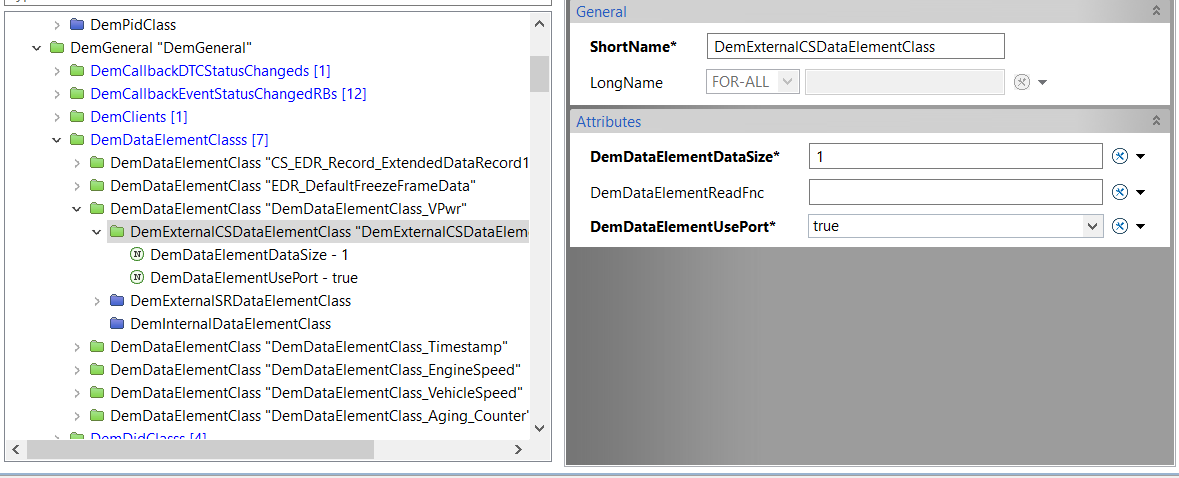
\includegraphics[width=\textwidth]{images/VPwr.png}
\caption{DEMDataElementClass configuration.}\label{fig:VPwr}
\end{figure}

Additionally, the users shall configure \textbf{SUSD\_C\_RunningResetWaitTime} for the serial data wait time after a running reset occurs, before going into the Fail-Soft state. By default, the configuration value will be 625 milliseconds.

The SUM\_SUSD shall also check if the single port feature is supported by verifying the configuration from SUM\_SSFM to see if this feature is enabled. In this way, the users should connect the SystemPowerMode\_FxI, SystemPowerMode\_FxFA, SystemBackupPowerMode\_FxI, and SystemBackupPowerMode\_FxFA interfaces to the SUM\_SSFM.

The users shall refer the DemDataElement class in the \textbf{SUSD\_DemDataElementClass\_VPwrSetEn CondDataSigRef} parameter and they shall connect the consequently generated port interface to the port "\textbf{PP\_CBReadData\_DemExternalCSDataElementClass}" defined in the SUSD module.

\subsection{Connections in Composition changes}
\begin{figure}[htp]
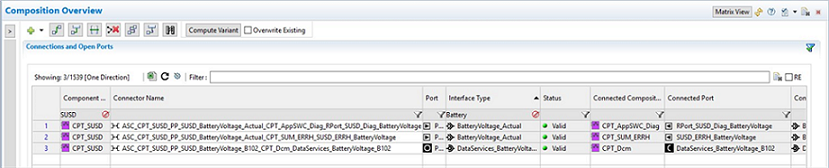
\includegraphics[width=\textwidth]{images/BatteryVoltageActualConnections.png}
\caption{BatteryVoltage\_Actual Connections.}\label{fig:BVAC}
\end{figure}
\begin{itemize}
\item Reconnection of AssemblyConnector between \textbf{(BatteryVoltage\_Actual)} PPort and \linebreak{\textbf{(SUSD\_ERRH\_BatteryVoltage)}} RPort of SUM\_ERRH might be required in Composition prototype, if available.


\item Reconnection of AssemblyConnector between \textbf{(BatteryVoltage\_Actual)} PPort and Application SWC might be required in Composition prototype, if available.


\item Reconnection of AssemblyConnector between \textbf{(BatteryVoltage\_Actual)} PPort and \linebreak{\textbf{(DataServices\_BatteryVoltage)}} RPort of DCM might be required in Composition prototype, if available.


\begin{figure}[htp]
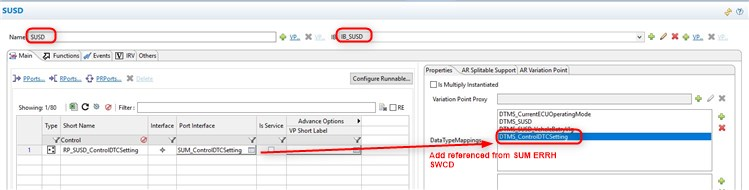
\includegraphics[width=\textwidth]{images/ControlDTCMappingERRH.jpg}
\caption{ControlDTC Mapping to ERRH.}\label{fig:CDME}
\end{figure}

\item Datatype Mapping Set of \textbf{(DTMS\_ControlDTCSetting)} is added to Internal Behavior of SUSD referenced from \textbf{ERRH}.

\end{itemize}

\subsection{SUSD\_BatteryVoltageRange}
\begin{figure}[h!]
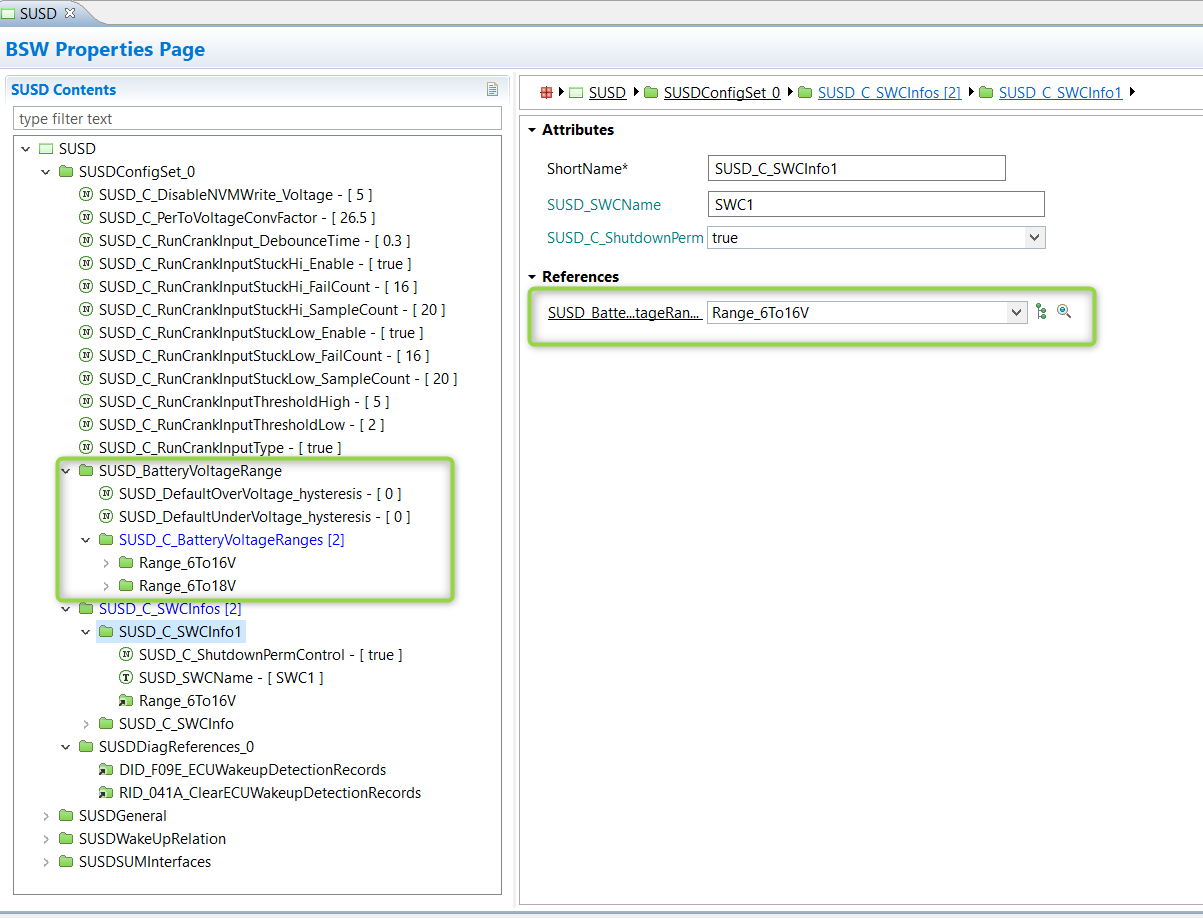
\includegraphics[width=\textwidth]{images/SUSDBatteryVoltageRange.png}
\caption{Battery Voltage Range.}\label{fig:BVR}
\end{figure}

The SUSD\_C\_BatteryVoltageRange is optional. Here are some notes about:

\begin{itemize}
\item PP\_SUSD\_DefaultBatteryVoltage\_MintoMax\_9Vto16V is always generated to used with 9V-16V range as default. \newline SUSD\_DefaultOverVoltage\_hysteresis
and SUSD\_DefaultOverVoltage\_hysteresis are 2 mandatory parameters and used correspondingly with this port to indicate voltage level.
\item For each configured SUSD\_C\_BatteryVoltageRange, a corresponding port \newline PP\_SUSD\_BatteryVoltage\_MintoMax\_<RangeName> is generated. 
\item If a SUSD\_C\_SWCInfo does not refer to any voltage range, it implicitly goes with 9V-16V default range and is notified about voltage level
by PP\_SUSD\_DefaultBatteryVoltage\_MintoMax\_9Vto16V port.
\end{itemize}

\subsection{ECU Operating Mode Port Configuration}
\label{subsec:ecuOperatingMode}
A mode switch port \textbf{PP\_SUSD\_ECUOperatingModeReq\_ECUOperatingMode} is provided by SUSD that needs to be properly configured in BswM to handle ECU state transitions. This port is used by SUSD to request ECU operating mode changes (RUN, BOOT, SLEEP, OFF states) from the BswM.

\begin{figure}[htp]
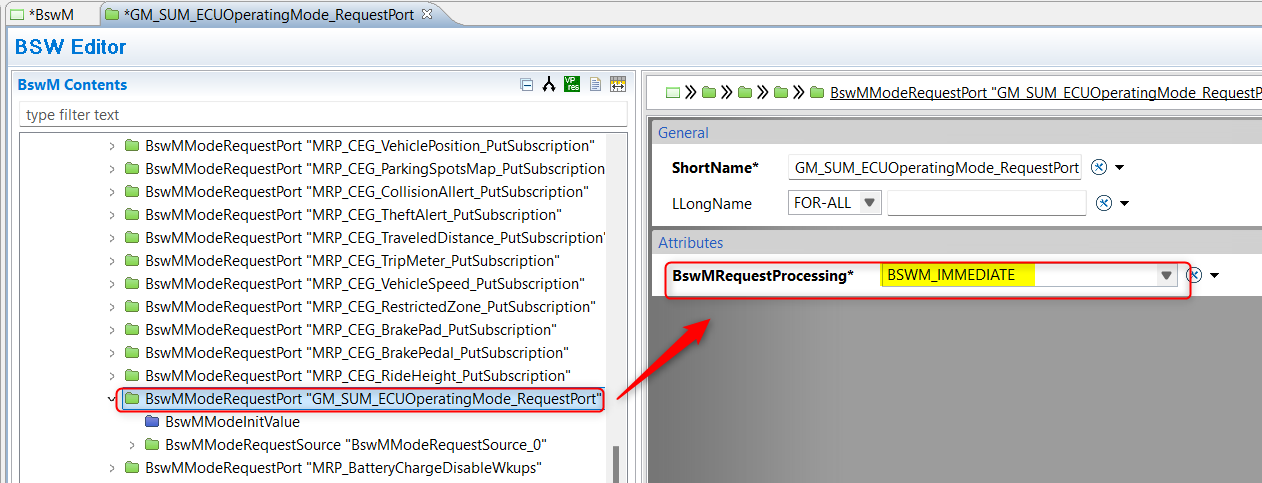
\includegraphics[width=\textwidth]{images/ECUOperatingMode.png}
\caption{ECU Operating Mode Port Configuration in BswM}\label{fig:ECUOperatingMode}
\end{figure}

To properly configure this mode port in BswM:

\begin{itemize}
\item Connect the SUSD mode switch port \textbf{PP\_SUSD\_ECUOperatingModeReq\_ECUOperatingMode} to the appropriate BswM mode request port
\item Configure the BswM mode switch action as \textbf{IMMEDIATE} on trigger to ensure timely ECU state transitions
\item Set up appropriate BswM rules to handle the different ECU operating modes (SUM\_INIT, SUM\_RUN, SUM\_BOOT, SUM\_SLEEP, SUM\_OFF)
\item Ensure that the mode switch triggers the necessary BSW module state changes and application layer notifications
\end{itemize}

The immediate trigger configuration is critical for proper power management and ensures that ECU state transitions occur without delay when requested by SUSD.

\subsection{Avoid Calibration Data Read Function Generation}\label{sec:cdata}
To avoid duplicates of calibration data read functions (\code{Rte_CData_SUSD_}), the configuration reported in Figure~\ref{fig:cdata} should be applied.
\begin{figure}[h!]
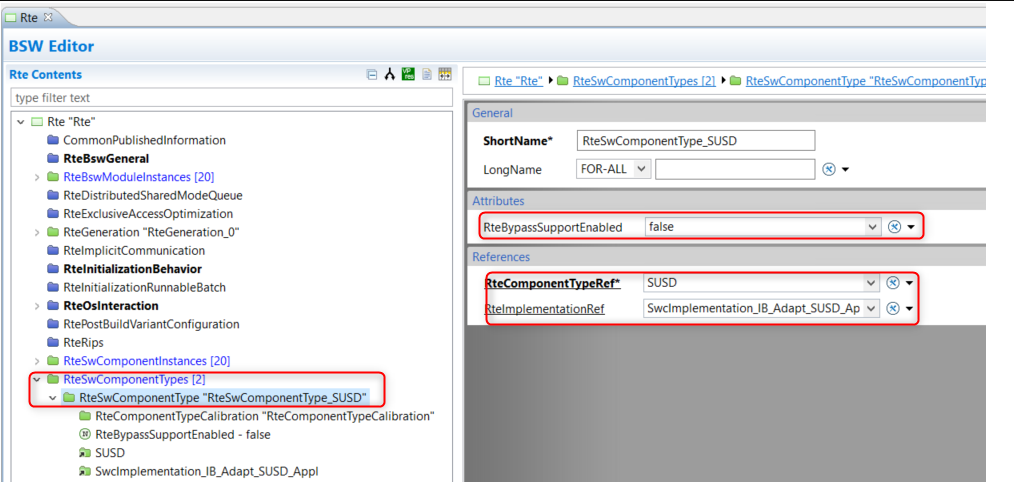
\includegraphics[width=\textwidth]{images/cdata}
\caption{Configuration needed to avoid duplicates of calibration data read functions.}\label{fig:cdata}
\end{figure}

\subsection{SUSD Initialization}
\label{sec:susdinit}

\subsubsection{SusdGenerateInitRunnable}
\begin{center}
	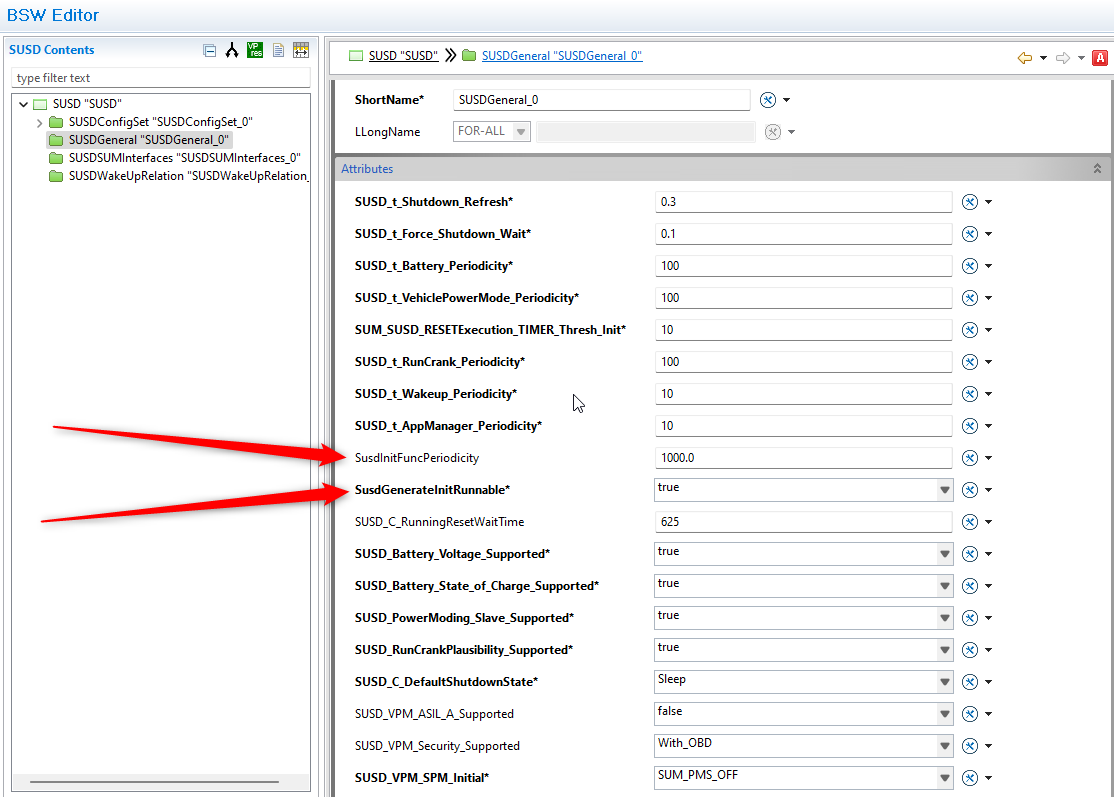
\includegraphics[width=\textwidth]{images/SusdGenerateInitRunnable}
\end{center}

The user needs to configure this parameter to determine whether to generate the initial runnable.
The SUSD\_Init function will be called just once at startup. 

If it is true, you shall need to configure parameter SusdInitFuncPeriodicity for the periodicity of SUSD init runnable. 
Otherwise, the SUSD\_Init functions shall be configured in the BswM init action list and to be called during the startup. 

\begin{center}
	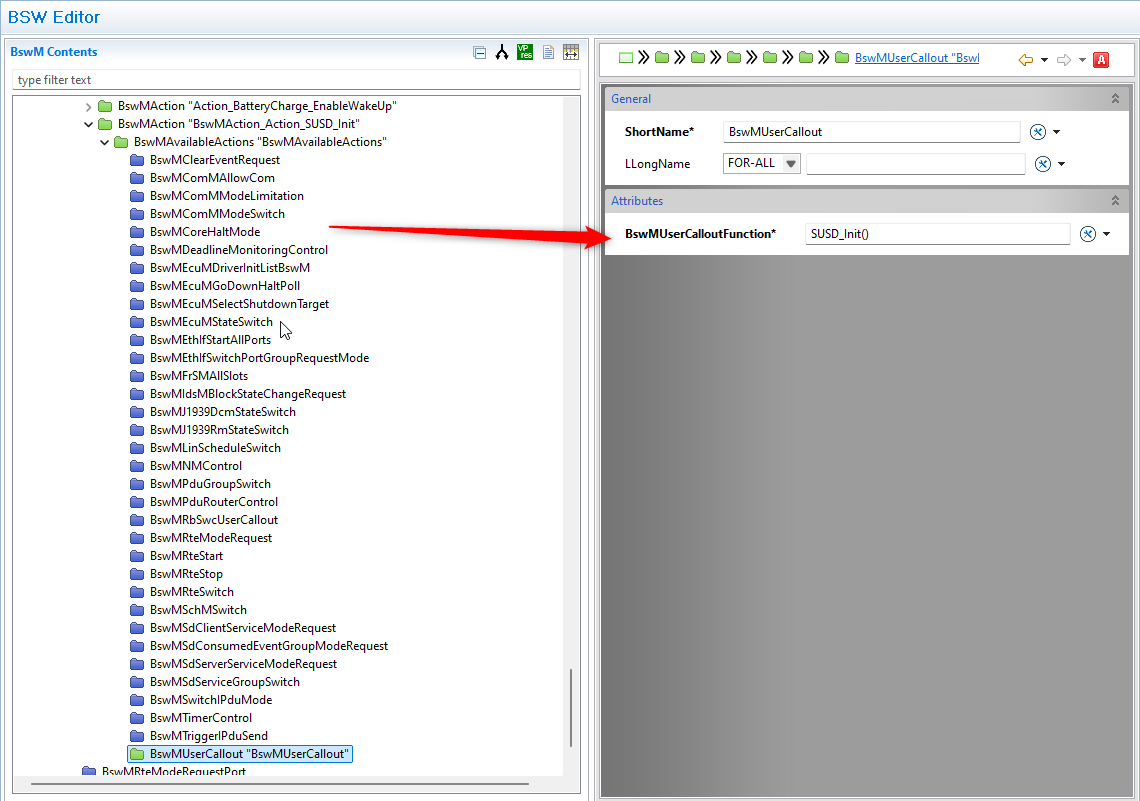
\includegraphics[width=\textwidth]{images/SUSD_Init_BswMActionList}
\end{center}

\begin{center}
	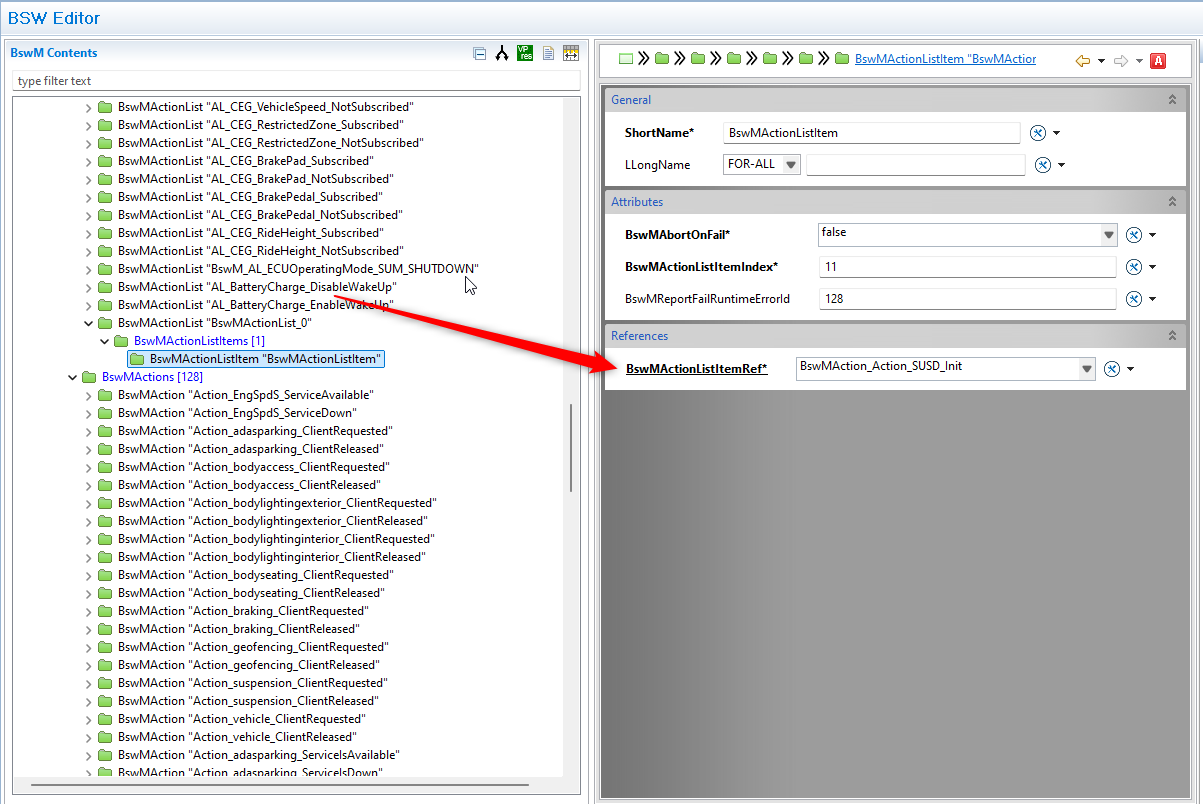
\includegraphics[width=\textwidth]{images/SUSD_Init_BswMActionListRef}
\end{center}

Ensure that this header file Sum\_Susd.h is included correctly in the BswM configuration file for declarations related to SUSD\_Init.

\begin{center}
	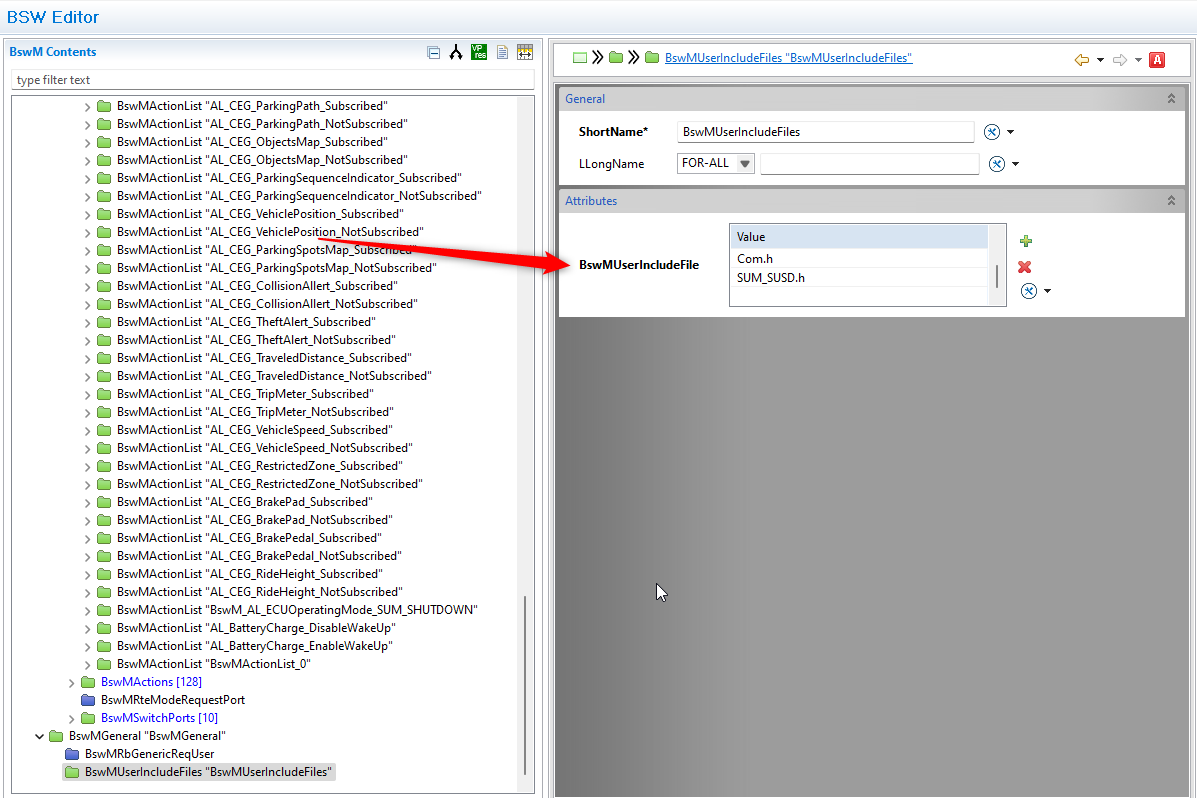
\includegraphics[width=\textwidth]{images/SUSD_Init_BswM_Included}
\end{center}

\subsubsection{SusdInitFuncPeriodicity}

Parameter defines the periodic fixed runnable for scheduling the SUSD initialization phase. By default, this timing period is 1000 (ms).

You shall need to map this generated runnable to the highest priority order task when the parameter SusdGenerateInitRunnable is set to true.
\chapter{Generic Component Interfaces}

\begin{figure}[htp]
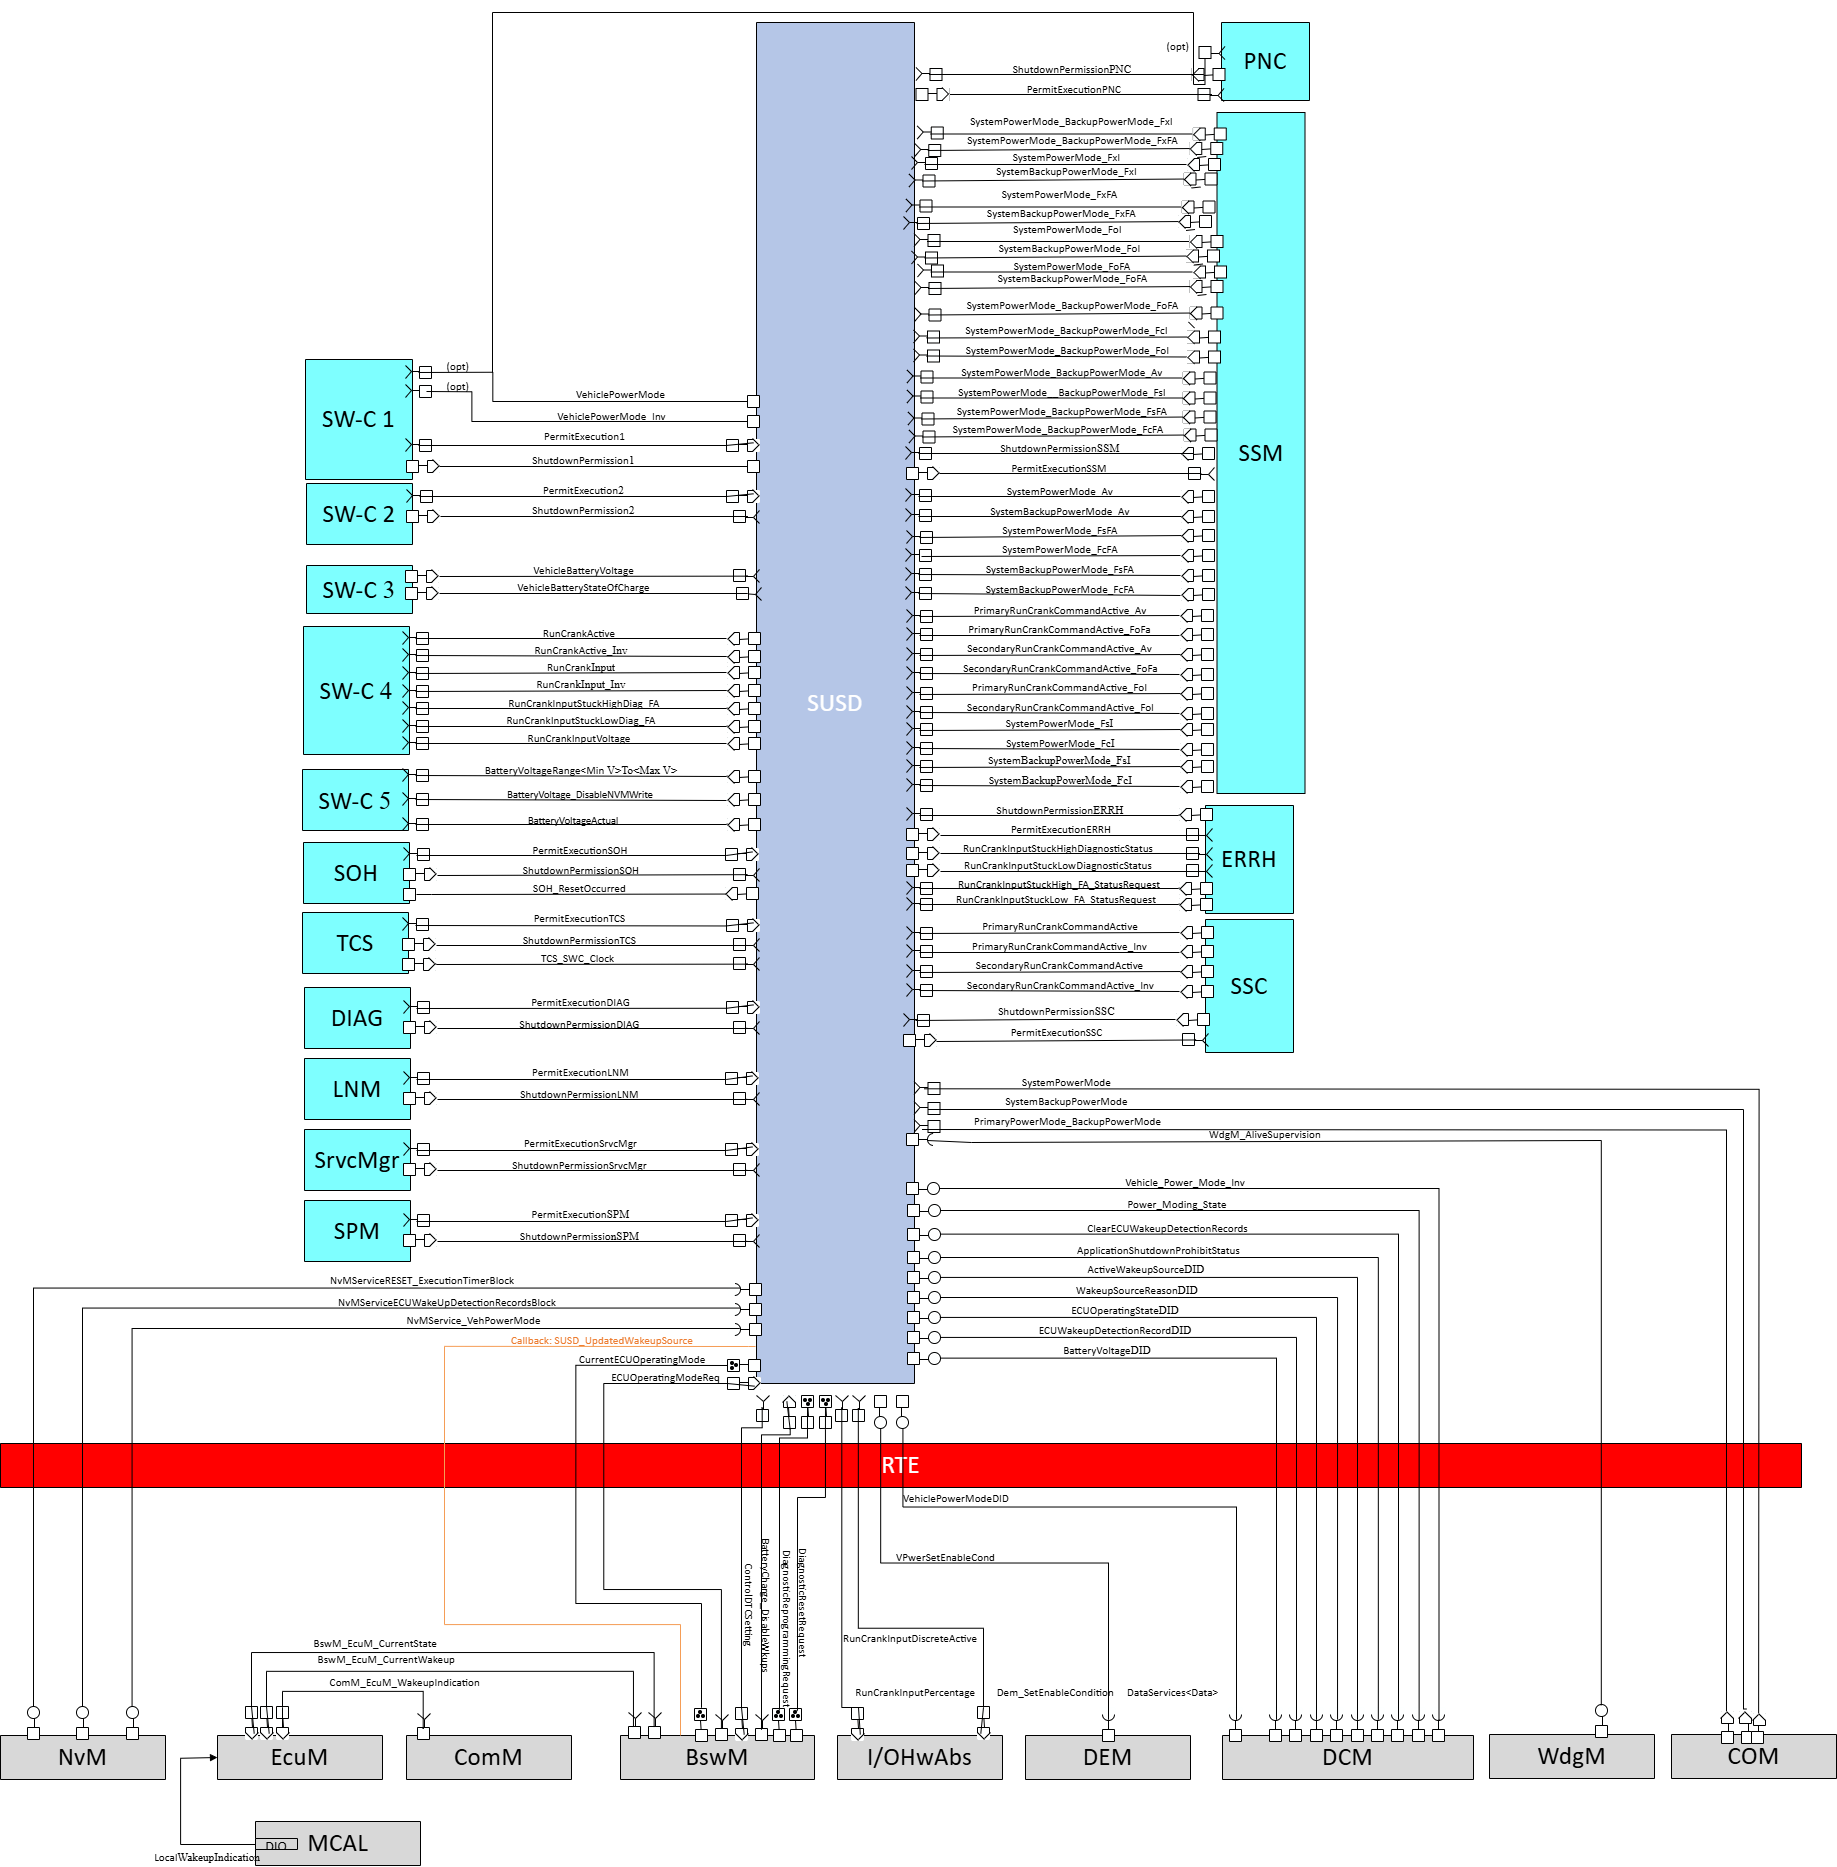
\includegraphics[width=\textwidth]{images/component.png}
\caption{RTA-SUM SUSD port interactions with the other modules.}\label{fig:component}
\end{figure}


\input{generated/tables/port_interfaces.tex}